\documentclass{mpaper}

\usepackage{enumitem}
\usepackage{color}
\usepackage{amsthm}
\usepackage{thmtools}

% \setlist[itemize]{leftmargin=*}
% \setlist[description]{leftmargin=*}

\newcommand{\specialcell}[2][c]{%
  \begin{tabular}[#1]{@{}c@{}}#2\end{tabular}}

\def\Item$#1${\item[] $\displaystyle#1$
   \hfill\refstepcounter{equation}(\theequation)}

\newtheorem{example}{Example}
\newtheorem{theorem}{Theorem}

\declaretheoremstyle[headfont=\bfseries]{solution}
\declaretheoremstyle[headfont=\normalfont]{normalhead}
\declaretheorem[style=normalhead, numbered=no]{question}
\declaretheorem[style=normalhead, numbered=no]{instance}
\declaretheorem[style=solution, numbered=no]{solution}


\begin{document}

\title{The Traveller's Problem}
\author{Iva Babukova}
\matricnum{2030458b}

\maketitle

% \begin{abstract}
% According to Simon Peyton Jones, an abstract should address
% four key questions. First, what is the problem that this
% paper tackles? Second, why is this an interesting problem?
% Third, what is the solution this paper proposes?
% Finally, why is the proposed solution a good one?
% \end{abstract}

\section{Introduction}
\label{intro}

The Traveller's Problem (TP) is a combinatorial optimisation problem whose extensions and variations are often encountered by travellers around the world.
Given a set of airports, a set of flights, a set of destinations that is a subset of the airports, and a special airport $A_{0}$, a solution to TP is a travel schedule that starts and finishes at $A_{0}$, visits all destinations and is in accordance with additional constraints specified by the traveller. For instance, the traveller may wish to spend a certain amount of days in each destination, to take a minimum number of connection flights, or to give minimum amount of money for flights.

% This work gives a formal description of TP and some of its main extensions, proves a result concerning its complexity, investigates existing methods to solve similar problems and presents two implemented TP models using Constraint Programming and Integer Programming, describes the random TP instances generator, that are going to be used for the empirical evaluation.

\subsection{Problem Formulation}
\label{sec:tpformulation}
Each instance of TP consists of:
\begin{enumerate}[topsep=0.1pt]
\setlength\itemsep{0.1em}
\item A set of airports $A = \{ A_{0},...,A_{n} \}$ for $n > 0$. Each airport $A_{i}$ $\in$ $A$ represents a location the traveller can begin their commute in, visit as a desired destination, or connect in on the way to their destination.

\item The trip starts and ends at the same airport $A_{0}$, which is referred to as the \textit{home point}.

\item The total travel time $T$, within which the traveller must have visited all destinations and returned to the home point. The first day is day 0.
 
\item A set of flights $F = \{ f_{0},...,f_{m} \}$. Each flight $f_{j}$ has:
\begin{itemize}[topsep=1pt]
\setlength\itemsep{0.1em}
\item departure airport $A^{d}_{j}$,
\item arrival airport $A^{a}_{j}$,
\item date $t_{j}$,
\item duration $\Delta_{j}$,
\item cost $c_{j}$,
\end{itemize} 
for some non-negative integer $j$ less than or equal to $n$.
The date $t_{j}$ is a positive rational number less than or equal to $T$ that shows at which day $f_{j}$ leaves its departure airport. The duration $\Delta{j}$ is a positive fraction that shows the amount of time that takes for flight $f_{j}$ to go from $A^{d}_{j}$ to $A^{a}_{j}$. The cost $c_{j}$ is a positive number that denotes the number of units of some currency $\epsilon$ that the traveller pays in order to be able to board flight $f_{j}$.

\item Each airport $A_{i}$ has a \textit{connection time} $C_{A_{i}}$, that is the time that takes to switch from any selected flight $f_{p}$ with $A^{a}_{p} = A_{i}$ to any selected flight $f_{q}$ with $A^{d}_{q} = A_{i}$, where $f_{q}$ is immediately after $f_{p}$ in a solution.

\item A set of \textit{destinations} $D = \{ D_{1},...,D_{l} \}$, $D \subseteq A$, $l \leq n$.
\end{enumerate}


A solution to any instance of TP is a sequence $s$ of $k$ valid flights, $ \langle f_{i_{1}}, f_{i_{2}},...,f_{i_{k}} \rangle \, \subseteq F$, also called a \textit{trip}. We say that $s$ is valid if the flights in $s$ have the following properties:

\begin{enumerate}
\item $A^{d}_{i_{1}} = A^{a}_{i_{k}} = A_{0}$
\item $ A^{a}_{i_{j}} = A^{d}_{i_{j+1}},  \quad 0 < j < k$
\item $ t_{i_{j}} + \Delta_{i_{j}} + C_{r} \leq t_{i_{j+1}}, \quad 0 < j \leq k, \quad r = A^{d}_{i_{j+1}}$
% david mentioned about possibly adding this as a hard constraint?
\item $t_{i_{k}} + \Delta_{i_{k}} \leq T$
\item $ \forall D_{p} \in D, \textrm{ } \exists \textrm{ } f_{i_{j}} \in s \textrm{, such that } A^{a}_{i_{j}} = D_{p} $
\end{enumerate}

In this work, we refer to these properties as \textit{trip properties}. Note that a valid sequence of flights may contain one or more flights to and from airports that are not destinations. Such airports are called \textit{connections}.

TP is NP-hard 
The \textit{optimization} version of TP (TPO) asks for an \textit{optimal} solution $s$ which minimizes the total sum of the prices of the flights in $s$, denoted by $c(s)$.

The \textit{decision} version of TP (TPD) asks whether there exists a valid sequence of flights $s$, such that $c(s)$ is less than or equal to some given integer $B$. The solution of this problem is a `yes' or `no' answer.

There exist a variety of additional constraints and extensions that can be added to TP. Our problem formulation has only presented the hard constraints which every valid solution to a TP instance must satisfy. In real-world problems, travellers may have additional preferences (soft constraints) and requirements (hard constraints) with regards to their travel. These are discussed in the next two sections.

\subsubsection{Hard Constraints}
\label{subsec:hardconstraints}
This section presents some additional constraints that might be imposed on a TP instance. If any of them is required, then a solution that does not satisfy the requirement is considered as invalid.

\begin{enumerate}
\item Travellers may wish to spend a certain amount of days at a given destination, specified by both upper and lower bounds. The days may additionally be constrained to be consecutive or not.

\item Travellers may require to spend a given date at a given destination, for example due to an event occurring on that date in this destination.

\item Travellers may require not to fly through a given airport more than once.
\end{enumerate}

\subsubsection{Soft Constraints}
\label{subsec:softconstraints}
It may be desirable to search for a solution that satisfies some of the following requirements:

\begin{enumerate}
\item Travellers may wish to spend a certain amount $\delta_{i}$ of days in each destination $D_{i}$, where $\delta_{i}$ may be specified as a lower or an upper bound.

\item Travellers may wish to avoid taking connection flights. In such requirement, we wish to maximise the number of flights to and from destinations.

\item Travellers may want to spend as little time on flying as possible. In such case, we wish to find a solution that minimises the sum of the durations of all flights.
\end{enumerate}

%% mention the problem with lexicographic optimisation and multi-objective opimisation
Note that we may have an instance for which all soft constraints can not be satisfied simultaneously. In such case, the traveller may be required to rank his requirements in an order of preference. The instance becomes a lexicographic optimisation problem, where we first optimise the highest ranked objective, and subject to this we optimise the second ranked objective and so on.
If all requirements are equally important for the traveller, we have to solve a multiobjective optimisation problem, where the objectives are all constraints required by the traveller. Each of the objectives is given a weight of importance. The problem is then to optimize the objective function, composed by the constraints, each of them multiplied by its weight. %Multiobjective and lexicographic optimisation problems are discussed later in this work.

Note that most of the aforementioned constraints can be viewed as either hard or soft, depending on the user requirements. It is therefore suggested that any attempt at an investigation of TP assumes as an additional non-functional requirement that any proposed model to solve TP is flexible and can be easily extended by adding, removing and modifying the aforementioned constraints.


% \section{Background Work}
% This section presents a detailed review of some existing methods to approach NP-hard problems.

% \subsection{Branch and Bound methods}

% \subsection{Integer Programming}
% Explain the Dantzig, Fulkerson IP formulation for TSP from the proposal

% \subsection{Constraint Programming}

\section{TP Solutions}
We have implemented two solutions for TP using Integer Programming (IP) and Constraints Programming (CP). This section presents the implemented models and our choice of IP and CP solvers.

% todo explain a bit about the flights and airports representation in the code.

\subsection{CP Solution}
\label{subsec:tpcp}

\subsubsection{CP Model}
Let $m = |F|$. We introduce an array $\mathcal{S}$ of size $m+1$ (indexed $0,1,...,m$) that represents the TP tour and a variable $z$ with domain $dom_{z} = \{1,...,m\}$ to denote the number of flights in the trip. If $\mathcal{S}[i] = j$, then flight $f_{j} \in F$ is the $(i+1)^{th}$ flight in the tour, for $(0 \leq i < m)$ and $(1 \leq j \leq m)$. To denote the end of the tour, we set $\mathcal{S}[z] = 0$. All subsequent variables in $\mathcal{S}$ will then have to be 0. Each variable $v$ in $\mathcal{S}$ is either 0, if no flight is taken at that step, or it is equal to some flight number, that is $dom_{v} = \{0,...,m\}$.

TP can then be formulated as the problem of minimising the objective function:

\begin{equation}
\label{eq:TPwithCPobj}
\sum^{m-1}_{i = 0} c_{\mathcal{S}[i]}
\end{equation}

subject to all constraints presented below.


The following constraint restricts that once the end of the trip is reached at some position $z$, no flights are further added to $\mathcal{S}$.
\begin{itemize}
\Item
$\mathcal{S}[i] > 0 \wedge \mathcal{S}[i+1] = 0 , \, (0 \leq i \leq z-1)$
\end{itemize}

The all-different constraint below enforces that every flight is taken only once \cite{Hoeve01}.
\begin{itemize}
\Item
$\textrm{allDiff}(\mathcal{S}[0],...,\mathcal{S}[z-1])$
\end{itemize}

The trip properties are enforced by the following five constraints, where constraint 1 corresponds to trip property (1), constraint 2 to trip property (2), etc:

\begin{enumerate}
% property 1:
\item
$dom_{\mathcal{S}[0]} = \{j \in \{1,...,m\} : A^{d}_{j} = A_{0}\}$
\item[]
$dom_{\mathcal{S}[z-1]} = \{j \in \{1,...,m\} : A^{a}_{j} = A_{0}\}$
% property 2:
\item
$dom_{\mathcal{S}[i]} = \{j \in \{1,...,m\} : A^{d}_{j} = A^{a}_{p}, \, p = \mathcal{S}[i-1]\},$
\item[]
$\forall i (1 \leq i < z)$
% property 3:
\item
$t_{p} + \Delta_{p} + C_{r} \leq t_{q}, \, p = \mathcal{S}[i], q = \mathcal{S}[i+1], r = A^{a}_{q},$
\item[]
$\forall i (1 \leq i < z)$
% property 4:
\item
$t_{q} + \Delta_{q} \leq T, \quad \textrm{ where } q = \mathcal{S}[z-1]$
% property 5:
\item
$\forall A_{k} \in D, \, |\{i: (0 \leq i < z) \wedge A^{a}_{\mathcal{S}[i]} = A_{k} \}| > 0 $
\end{enumerate}

Constraint 1 restricts the domains of the first and the $(z-1)^{th}$ variable in $\mathcal{S}$ to contain only flights that depart from/arrive at the home point. For constraint 2, the domain of each variable in $\mathcal{S}$ is set to include only flights that depart from the arrival airport of the previous flight. Constraint 5 restricts that the number of the flights that arrive at every destination in the trip is positive. % todo: the actual implementation of this might be a different constraint

\subsubsection{Choice of CP Solver}
We use Choco 4.

% \subsection{IP Solution}
% Most of the constraints for the TP CP model need modification in order to be applicable to an IP model. In particular, IP does not allow for ``if-then'', ``all-different'' and other constraints that are not integer linear inequalities. The model described in this section is a modification of the TP CP model that gives constraints in the form of integer linear inequalities, which we also refer to as \textit{constraints}.

% \subsubsection{IP Model}
% Let $m = |F|$. We introduce a variable $x_{i,j}$ for every $i \in \{0,...,m-1\}$ and  $j \in \{0,...,m-1\}$, such that $x_{i,j} = 1$ if $(i+1)^{th}$ flight is $f_{j+1}$ or 0 otherwise. This variable is somewhat similar to $\mathcal{S}$, used for the CP model, where $\mathcal{S}[i] = p$ is equivalent to $x_{i,p} = 1$. In addition, we introduce a variable $x_{m,m} = 1$, where flight $f_{m}$ is a ``special'' flight with duration $\Delta_{j} = 0$, date $t_{j} = T$, departure and arrival airports $A^{d}_{j} = A^{a}_{j} = A_{0}$ and cost $c_{j} = 0$ This special flight is used for enforcing the valid ending of the trip at the home point without the need of an additional variable, as it is the case with $z$ in the CP model. The special flight can be scheduled more than once. It is added to $F$ and the new size of $F$ is $m^\prime = m + 1$. The first occurrence of $f_m$ marks the end of the trip.

% The variable $x_{i,j}$ is implemented as a two dimensional matrix of size $m^\prime \times m^\prime$.

% todo explain why we need the special flight

% The objective function of TP is to minimise:

% \begin{equation}
% \label{eq:TPwithIPobj}
% \sum^{m-1}_{i=0} \sum^{m}_{j=0} c_{j} x_{i,j}
% \end{equation}

% subject to the constraints presented below.

% \textcolor{red}{The first of the following three constraints restricts that there is exactly one scheduled flight at each step by adding a requirement that each row $i$ in the matrix has one 1. The second constraint imposes that each flight is taken at most once. The first and the second constraint are equivalent to the all-different constraint used in the CP model. The second and the third constraint allow for constructing flight schedules that do not use all flights in $F$.}

% \begin{itemize}
% \Item
% $\forall i \, (0 \leq i < m), \quad \sum^{m}_{j = 0} x_{i,j} = 1 $
% \Item
% $\textcolor{red}{\forall j \, (0 \leq j < m), \quad \sum^{m-1}_{i = 0}x_{i,j} \leq 1} $
% \Item
% $\textcolor{red}{\sum_{i=0}^{i = m} x_{i,m} \geq 1 }$
% \end{itemize}

% \textcolor{red}{The following constraint enforces that once the trip is ended, no more flights can be scheduled. Assume that flight $z-1$ is the final flight returning to $A_{0}$, where $1 \leq z \leq m$. The constraint adds $m-z+1$ many $f_{m}$ flights, so that the variables $x_{z,m},...,x_{m,m}$ are all equal to 1.}
% \begin{itemize}
% \color{red}
% \Item 
% $\forall i \, (1 \leq i < m), \quad \sum_{j=0}^{j<m} x_{i-1,j} \geq  \sum_{j=0}^{j<m} x_{i,j}$
% \end{itemize}

% Each of the trip properties is expressed as an integer linear inequality as follows.

%We do not add connection time when connecting from $A_{0}$ to $A_{0}$ as part of these flights.

% The following two constraints enforce trip property (1). The first flight is restricted to depart from the home point and the last flight arrives at the home point. From trip property (2) it follows that there must exist some $z < m$, $x_{z,j} = 1$, for which $j \neq m$ and $A^{a}_{j} = A_{0}$. Thus, $A^{a}_{j} = A_{0}$ is indirectly enforced.

% \begin{itemize}
% % property 1:
% \Item
% $\sum_{j \in S_{1}} x_{0,j} = 1, \, \textrm{where}$
% \item[]
% $ S_{1} = \{j \in \{0,...,m-1\} : A^{d}_{j} = A_{0}\}$
% \Item
% $x_{m,m} = 1$
% \end{itemize}

% Property (2) is enforced by defining two sets of flights $S_{1}$ and $S_{2}$, such that all flights in $S_{2}$ depart from the arrival airport of $S_{1}$. Every flight is restricted to depart always from the arrival airport of the previous taken flight.

% \begin{itemize}
% % property 2:
% \Item
% $\forall i \, (1 \leq i \leq m) \wedge \forall y \in A, \, \sum_{j \in S_{1}} x_{i-1,j} = \sum_{j^{\prime} \in S_{2}} x_{i,j^{\prime}},$
% \item[]
% $\textrm{where:}$
% \item[]
% $S_{1} = \{j \in \{0,...,m\} : A^{a}_{j} = y\},$
% \item[]
% $S_{2} = \{j^{\prime} \in \{0,...,m\} : A^{d}_{j^{\prime}} = y\}$
% \end{itemize}

% Trip properties (3) and (4) are represented by one constraint, which enforces that every flight $f_{j}$ cannot depart until the previous flight $f_{j^{\prime}}$ has arrived, adding connection time, if needed.

% \begin{itemize}
% % property 3 and 4:
% \Item
% $\forall i \, (0 \leq i < m), \, \forall j \, (0 \leq j \leq m):$
% \item[]
% $x_{i+1,j} + \sum_{j^{\prime} \in F^{\prime}} x_{i,j^{\prime}} \leq 1, \, \textrm{where:} $
% \item[]
% $F^{\prime} = \{j^{\prime} : f_{j^{\prime}} \in F \wedge t_{j^{\prime}} + \Delta_{j^{\prime}} + C^{\prime}_{r} > t_{j} \},$
% \item[]
% $C^{\prime}_{r} =   \begin{cases}
% 0, \quad \textrm{ if } j=m \\
% C_{A^{a}_{j^{\prime}}}, \quad \textrm{ otherwise}
% \end{cases}
% $
% \end{itemize}

% % property 5:
% Trip property (5) is enforced by restricting that all destination airports must be visited by at least one flight:

% \begin{itemize}
% \Item
% $\forall A_{k} \in D, \, \sum_{i=0}^{m-1} \sum_{j \in F_{k}} x_{i,j} \geq 1, \, \textrm{where:} $
% \item[]
% $F_{k}= \{j : f_{j}\in F \wedge A^{a}_{j} = A_{k}\} $
% \end{itemize}

% \subsubsection{Choice of IP Solver}

% \subsection{Soft and Hard Constraints}

%todo: Explain the implementation of the soft and hard constraints.


\subsubsection{Hard Constraint 2}
Hard constraint 2 (HC2) in Section \ref{subsec:hardconstraints} is implemented in the CP model as follows. Let $P = \{p_{1},...,p_{h}\}$ denote the list of every HC2 for a given TP instance $\pi$. Each HC2 is represented as a pair $p_{r} = \langle A_{k_{r}}, t_{i_r} \rangle \in P$ for $0 \leq r \leq h \leq |D|$, where the traveller must be at destination $A_{k_r} \in D$ at date $t_{i_r} < T$.

We introduce an array $\mathcal{D}$ of size $h$. The domain of each variable in $\mathcal{D}$ is $\{1,...,m\}$. If $\mathcal{D}[r] = i$, then the flight at position $\mathcal{S}[i]$ departs from $A_{k_r}$ at least one day after date $t_{i}$ \footnote{It is assumed that the traveller wants to stay at least for a day after the required date. Ideally, the solver should allow for taking this as an input parameter.} and the flight $\mathcal{S}[i-1]$ arrives at $A_{k}$ before date $t_{i_r}$, satisfying $p_{r}$. This is achieved by the following constraints:

\begin{itemize}
\Item
$\forall \, p_{r} \in P, \, \exists \, i \, (0 < i < m):$
\item[]
$\mathcal{D}[r] = i \wedge dom_{\mathcal{S}[i-1]} = S_{1} \wedge dom_{\mathcal{S}[i]} = S_{2}, \textrm{ where:}$
\item[]
$S_{1} = \{j : f_j \in F \wedge A^{a}_{j} = A_{k_{r}} \wedge t_{j} + \Delta_{j} < t_{i_r} \},$
\item[]
$S_{2} = \{j^\prime : f_{j^\prime} \in F \wedge A{^d}_{j^\prime} = A_{k_{r}} \wedge t_{j^\prime} > t_{i_r} + 1 \}$
\end{itemize}

\begin{itemize}
\Item
$\textrm{allDiff}(\mathcal{D}[1],...,\mathcal{D}[h])$
\end{itemize}

\subsection{Objective Functions}

\section{TP Datasets}
This section is dedicated to the process of obtaining all TP instances used later during the evaluation.

\subsection{Data Format}
Each TP instance is represented as JSON formatted file, as shown in Figure \ref{fig:dataFormat}. We have chosen JSON over other possible representations for its ease of use, flexibility and wide support for most programming languages.

\begin{figure}
\centering
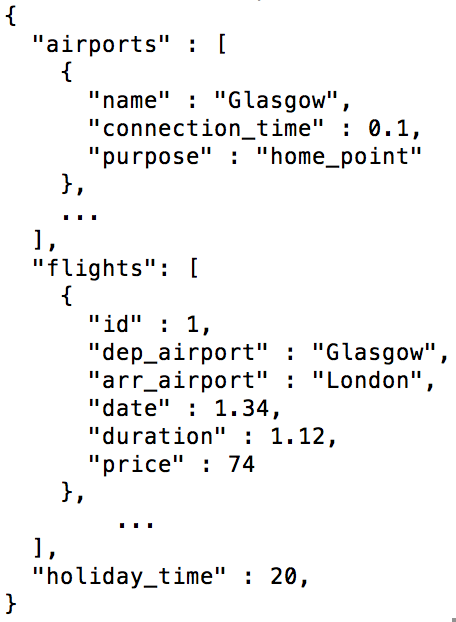
\includegraphics[height=5.5cm, width=4cm]{images/dataFormat.png}
\caption{\label{fig:dataFormat}The format of TP instances.}
\end{figure}

\subsection{Random Datasets}
In order to generate random TP instances, we have written a custom data generator $G$. This section discusses its implementation.

Program $G$ is written in Python. Given a number of flights $m$, a number of airports $n$, a number of destinations $d$, a holiday time $T$ and a unique id $i$, it returns a TP instance formatted as described in the previous section.

TP instances are generated using the following steps. First, $G$ chooses $n$ airports, each with randomly assigned connection time between 0.01 and 1 and a unique string as name. From these airports, one is chosen as a home point and $d$ are chosen as destinations.

Next, $G$ generates a list $l$ consisting of the names of all destinations and the home point. The first and the last element in $l$ is the name of the home point. The other elements are all destinations, ordered randomly.

As a third step, $G$ creates a list of flights $l_f$ that forms a valid trip and visit all airports in the specified order in $l$.

The fourth step consists of dividing each flight in $l_f$ in two flights until either the size of $l_f$ reaches $m$ or no flight can be further divided. For each flight $f_j \in l_f$ we create two flights $f_j1$ and $f_j2$, such that:

\begin{itemize}
\item $A^d_{j1} = A^d_j$,
\item $A^a_{j2} = A^a_j$,
\item $A^a_{j1} = A^d_{j2} = A_{k}$, where $A_{k}$ is chosen randomly from $A$,
\item $t_{j1} + \Delta_{j1} + C_{A_{k}} \leq t_{j2}$,
\item $t_{j1} \geq t_j$, and
\item $t_{j2} + \Delta_{j2} \leq t_j + \Delta_j$
\end{itemize}

Step five consists of generating flights with random arrival and departure airports, random date that is less than $T$ and random duration. It is executed only if the number of flights in $l_f$ is less than $m$ and until it reaches $m$.

Without loss of generality, the cost of each flight generated after either of the aforementioned steps is configured to be a random number from 1 to 200.

\subsection{Skyscanner Flights Data}
% If we manage to get it, write how we make it usable. If we don't manage to get it, write that we wanted to do this and tried hard.

% \section{Empirical Study}

% Graphs are always good. I recommend getting to grips with Matlab, R or
% gnuplot rather than exporting horribly Excel bitmapped graphs.


% \begin{quotation}
%  The Assyrian came down like the wolf on the fold,
%  And his cohorts were gleaming in purple and gold;
%  And the sheen of their spears was like stars on the sea,
%  When the blue wave rolls nightly on deep Galilee.

%  Like the leaves of the forest when Summer is green,
%  That host with their banners at sunset were seen:
%  Like the leaves of the forest when Autumn hath blown,
%  That host on the morrow lay withered and strown.
% \end{quotation}

% \section{Conclusion}

% The standard Lorem Ipsum passage, used since the 1500s

% ``Lorem ipsum dolor sit amet, consectetur adipisicing elit, sed do eiusmod tempor incididunt ut labore et dolore magna aliqua. Ut enim ad minim veniam, quis nostrud exercitation ullamco laboris nisi ut aliquip ex ea commodo consequat. Duis aute irure dolor in reprehenderit in voluptate velit esse cillum dolore eu fugiat nulla pariatur. Excepteur sint occaecat cupidatat non proident, sunt in culpa qui officia deserunt mollit anim id est laborum.''
% \vskip8pt \noindent
% {\bf Acknowledgments.}
% This is optional; it is a location for you to thank people

% \clearpage

\bibliographystyle{abbrv}
\bibliography{example}

% \clearpage

\appendix

\section{Investigated Problems}
\label{npcompleteproblems}

\begin{enumerate}
\item \textbf{Travelling Salesman Problem \textsuperscript{*} (TSP) \footnote{Note that TSP is a special case of VRP when only one vehicle is allowed.}}
\begin{instance}
Set $A$ of $n$ cities, distance $d(A_{i}, A_{j})$ between each pair of cities $A_{i}$, $A_{j}$ $\in$ $A$, positive integer $B$.
\end{instance}

\begin{question}
Is there a tour of $A$ having length $B$ or less, i.e., a permutation of cities $\gamma = \langle A_{\pi_{1}},...,A_{\pi_{n}} \rangle $ of $A$ such that the total travel distance $L_{\gamma}$:
$$L_{\gamma} = \bigg( \sum_{i=1}^{n-1} d(A_{\pi_{i}}, A_{\pi_{i+1}}) \bigg) + d(A_{\pi_{n}}, A_{\pi_{1}}) \leq B \quad \textrm{?}$$
\end{question}
\end{enumerate}

\section{Complexity of TP}
\label{appendix:tpcomplexity}
\begin{theorem}
TPD is NP-complete.
\end{theorem}

\begin{proof}
This proof first shows the membership of TPD in the NP class of problems. Second, we prove the NP-hardness of TP by constructing a polynomial-time reduction from a known NP-complete problem $\Pi$ to TPD, where $\Pi$ is chosen to be TSP, defined in Section \ref{npcompleteproblems}. Its NP-hardness follows by a reduction from the Hamiltonian Cycle problem. The proof is presented by
\cite{thebible}.

Given an instance of TPD and $s$, which is a sequence of flights from $F$, we can write an algorithm that checks in polynomial time whether $s$ is a solution. To accept or reject validity, the algorithm only needs to traverse $s$ and check that it satisfies all required properties. Therefore, TP is in NP.

Let $\pi$ be an instance of TSP. Let $\pi^{\prime}$ be an instance of TPD with the following properties:
\begin{itemize}
\item The set of airports in $\pi^{\prime}$ is identical to the set of cities in $\pi$ and it is similarly denoted as $A$ (a city in $\pi$ is called an airport in $\pi^{\prime}$). Airport $A_{1}$ is the home point.
\item Each airport in $A$ is also a destination.
\item The connection time $C_{A_{i}}$ for each airport $A_{i}$ is equal to 0.
\item $T$ is equal to $n$.
\item Let $C$ be the Cartesian product of the airports in $A$ with itself, that is $C = A \times A$ = \{($A_{i}, A_{j}$) : $A_{i}$ $\in$ $A$, $A_{j}$ $\in$ $A$, $i \neq j$\}. Then $F$ is a set of flights, such that for every ($A_{i}, A_{j}$) $\in$ $C$, there exists a flight $f_{k}$ in $F$, such that $A^{d}_{k} = A_{i}$ and $A^{a}_{k} = A_{j}$ for every date $0 \leq t < T$.
\item For every $f_{k}$ $\in$ $F$, $c_{k}$ is equal to $d(A^{d}_{k}, A^{a}_{k})$ in $\pi$. Therefore, the flight costs also satisfy the triangle inequality.
\item For every $f_{k}$ $\in$ $F$, $\Delta_{k}$ = 1.
\item $B$ is the upper bound on the allowed total cost.
\end{itemize}

%% TSP solution => also TP solution

Suppose that $\gamma$ = $ \langle A_{i_{1}}, A_{i_{2}},...,A_{i_{n}} \rangle $ is a solution to $\pi$, where $\langle i_{1},...,i_{n} \rangle$ is a permutation of $\langle 1,...,n \rangle $ and the total travel distance $L_{\gamma} \leq B$. Without loss of generality, assume that $i_{1} = 1$. In $\pi^{\prime}$, $\gamma$ is equivalent to the order of visited airports by some sequence of flights $s$ = $ \langle f_{j_{1}}, f_{j_{2}},...f_{j_{n}} \rangle $, such that for each $p$  $(1 \leq p \leq n)$ there exists $q$ $(1 \leq q \leq n)$ such that $A^{d}_{j_{q}} = A_{i_{p}}$ and $A^{a}_{j_{q}} = A_{i_{p+1}}$, where subscripts are taken modulo $n$. Therefore, $s$ satisfies property (1) of a valid solution. For each $q$ $(1 \leq q \leq n)$, $A^{a}_{j_{q}} = A^{d}_{j_{q+1}}$ and $t_{j_{q}} = q - 1$.  We know that such flights exist in $F$ by the construction of the set $F$.

From the construction of $s$, it follows that property (2) also holds. Properties (3) and (4) also hold, since we have chosen flights from $F$ such that for every $f_{j_{q}}$ $\in$ $s$, $t_{j_{q}} = q - 1$ ($(1 \leq q \leq n)$). Property (5) is satisfied, since all airports in $A$ are destinations.

Since the cost of every flight in $F$ is equal to the distance between the two cities in $\pi$ that correspond to its departure and arrival airport, it follows that $c(s) = L_{\gamma} \leq B$.

The sequence $s$ satisfies all requirements for a valid solution to $\pi^{\prime}$. Therefore, a solution of $\pi$ is also a solution to $\pi^{\prime}$.

Conversely, suppose that $s = \langle f_{j_{1}},...,f_{j_{k}} \rangle $ is a solution to $\pi^{\prime}$, where the flights in $s$ visit destinations in the sequence $\gamma^{\prime}$ = $\langle A_{i_{1}}, A_{i_{2}},...,A_{i_{m}} \rangle$. We will prove that $\gamma^{\prime}$ is a solution of $\pi$.

By construction of $\pi^{\prime}$, all airports in $A$ are also destinations. Therefore, $\gamma^{\prime}$ contains all cities in $A$, that is $m \geq n$. Suppose that $m > n$ and an arbitrary airport $A_{p}$ $(1 \leq p < n)$ is included more than once in $\gamma^{\prime}$. Then $s$ must contain more than one flight with arrival airport equal to $A_{p}$. 
The duration of each flight in $\pi^{\prime}$ is one day. Therefore, for every $q$ $(1 \leq q < n - 1)$, $t_{j_{q+1}} = q$. Since the traveller has only $n$ days of total travel time, and $s$ is restricted to contain exactly $n$ flights, that is $k = n$. The only way to visit $n$ distinct destinations, given $n$ flights is that all flights in $s$ have unique arrival airports. Assuming that $A_{p}$ is visited more than once means that there is more than one flight with arrival airport equal to $A_{p}$, which is a contradiction. Therefore, $m = n$ and each airport in $A$ is visited exactly once.

From the properties of $s$ it follows that $A^{d}_{j_{1}} = A^{a}_{j_{n}} = A_{1}$. Therefore, $\gamma^{\prime}$ is a cycle of size $n$. We know that $c(s) \leq B$. We assigned a cost of each flight $f_{k}$ in $F$ to be equal to $d(A^{d}_{k}, A^{a}_{k})$ in $\pi$. Therefore, the total travel distance $L_{\gamma^{\prime}} = c(s)$ which is less than or equal to $B$.

According to the specifications of $\pi$, $\gamma^{\prime}$ is a solution to $\pi$. Therefore, a solution to $\pi^{\prime}$ is also a solution to $\pi$.

The transformation from a TSP instance to an instance of TPD can be done in polynomial time. For each of the $n$($n$-1)/2 distances d($A_{i}$, $A_{j}$) that must be specified in $\pi$, it is sufficient to check that the same cost is assigned to the flights from $A_{i}$ to $A_{j}$ for all dates.

Therefore, TP is in NP and the decision version of TSP can be reduced to TPD in polynomial time, from which it follows that TPD is NP-complete.
\end{proof}

\end{document}
